\section{Dominio del problema}
    \subsection{Wiki, Mediawiki y Wikimedia}

        El término wiki proviene de la raíz Hawaiana \say{wiki}, que significa \say{rápido}, y fue propuesto por Ward Cunningham, quien a su vez define los sitios web wiki como "La base de datos más simple que puede existir" \cite{WhatIsWiki}. Con el tiempo este concepto fue evolucionando, y en la actualidad cuando hablamos de wiki nos referimos a un sitio web que permite a sus usuarios colaborar en su estructura y contenido. Estos sitios webs son impulsados por el motor wiki, también llamado MediaWiki, el cual es un Sistema Manejador de Contenido (CMS) que permite a los usuarios colaborar en el sitio web sin la necesidad de tener permisos de dueño o líder.

        La enciclopedia Wikipedia es el sitio web más popular basado en wiki, que a su vez forma parte del movimiento Wikimedia, el cual incluye otros proyectos interrelacionados, tales como: Wiktionary, Wikiquote, Wikibooks, Wikisource, entre otros, cuyo propósito es usar el poder colaborativo de internet, y el concepto wiki, para compartir conocimiento gratuito de cualquier tipo.
     
    \subsection{Filosofía de wiki}

        En la actualidad, gracias a la evolución del internet, la información es considerada virtualmente ubicua y en constante cambio, y lo que realmente ofrece valor es la capacidad individual de sintetizar esa información y relacionarla. Como resultado de esto surge la filosofía wiki, en donde la información se comparte, y el conocimiento no se crea, sino se co-crea de forma colaborativa.

        El concepto de la filosofía de wiki y el software utilizado para crear estos sitios web están intrínsecamente relacionados, y no se podría poner en práctica lo primero sin lo segundo. Esto es así debido a que el software debe proporcionar el medio para que pueda existir esa construcción colectiva de conocimiento, que es indispensable en la filosofía wiki.
        
        Algunas de las características de software de los sitios web que hacen uso de esta filosofía son: 
    
        \begin{enumerate}
            \item Cualquiera puede cambiar cualquier cosa
            \item Usan un sistema de marcas hipertextuales simplificadas, lo que resulta imprescindible para hacer posible la colaboración.
            \item No posee una estructura predefinida a la que se tengan que acomodar los usuarios, lo que otorga flexibilidad.
        \end{enumerate}

    \subsection{Moderación de contenido en Wikipedia}

        El principal problema que maneja Wikipedia en cuanto a moderación de contenido viene como resultado de su propia filosofía "todos pueden editar", lo que conlleva a múltiples problemas tales como: vandalismo, escritura pobre, una mala estructura de página, peleas de edición, entre otras cosas. Por esta razón no existe una solución única para acabar con la existencia de \say{mal} contenido en Wikipedia, y es indispensable el uso de participación humana en procesos de moderación que implican complejos desafíos técnicos y éticos.

        Una de las formas que tiene Wikipedia de detectar vandalismo es usando las estadísticas de los artículos para verificar si hay una gran cantidad de ediciones de un articulo en un periodo muy corto de tiempo, o si estas revisiones vienen de la misma dirección IP, bloqueando o baneando las direcciones IP como método de reducción de vandalismo. Sin embargo, el bloqueo de IPs es en sí mismo un método que resulta contradictorio para el núcleo principal de la filosofía de wiki: "todos pueden editar", por lo que el bloqueo de IPs es utilizado siempre como última alternativa contra el vandalismo.

        
    \subsection{Watcher}
        
        El concepto de watcher en Wikipedia no difiere mucho de las demás paginas que aplican el mismo sistema, siendo este una forma que permite al usuario obtener información de presencia de aquellas paginas que se encuentran en su watchlist.

        En el ámbito de Wikipedia la información de presencia de una pagina se refiere a los cambios recientes hechos a dicha pagina, desplegados de forma simplificada en conjunto con todas las demás páginas de interés para el usuario.
       
    \subsection{Wikipedia como ejemplo práctico}

        Wikipedia es un sitio web que permite a sus usuarios obtener conocimiento de una gran variedad de temas, siendo la enciclopedia online mas grande que existe; esto se debe a su naturaleza colaborativa que permite a cualquier persona aportar conocimiento escribiendo o editando artículos. Al mismo tiempo, los grupos encargados de realizar la moderación de contenido no son suficientes para asegurar que todo el contenido que existe en el sitio web sea verídico, haciendo de Wikipedia un sitio web con contenido no confiable por las entidades académicas.

    \subsection{Visualización científica}

        La visualización científica es una rama interdisciplinaria de la ciencia cuyo propósito es la visualización de fenómenos científicos. Su propósito es ilustrar gráficamente datos científicos para permitir a los científicos comprender, ilustrar y obtener información de los datos.

        La visualización de datos científicos, clasificada como visualización científica en 2D o 3D, utiliza técnicas de una variedad de campos, incluido el procesamiento de imágenes, la animación por computadora, la visión por computadora, el procesamiento de señales, los gráficos por computadora, la interacción humano-computadora y el diseño asistido por computadora.


    \subsubsection{Métodos de visualización cientifica}

        Los métodos para la visualización científica 2D y la visualización científica 3D incorporaron cada vez más gráficos por computadora a medida que la disciplina maduraba, siendo los campos vectoriales y campos escalares de datos medidos y simulaciones por computadora las principales aplicaciones.

        Los métodos principales para la visualización científica en 3D de campos escalares son las isosuperficies y la representación de volumen, y los métodos principales para la visualización científica en 3D de campos vectoriales incluyen el rastreo de partículas, los glifos y la convolución integral de línea; los métodos principales para la visualización científica 2D de campos escalares son el dibujo de líneas de contorno y el mapeo de colores, mientras que los métodos principales para la visualización científica 2D de campos vectoriales incluyen glifos y líneas aerodinámicas o convolución integral de línea.
        
        Algunas herramientas de visualización científica incluyen:

        \begin{itemize}

            \item \textbf{Animación por computadora} 

            el proceso de creación de imágenes animadas generadas digitalmente. \hfill 

            \item \textbf{Simulación por computadora} 

            Simulación por computadora: se refiere a los intentos de una red de computadoras o un programa de computadora para simular los resultados de un modelo matemático asociado con un sistema en particular. \hfill 

            \item \textbf{Representación de superficie} 

            el proceso automático mediante el cual un programa de computadora genera una imagen a partir de un modelo 2D o 3D; las técnicas incluyen representación de línea de exploración, trazado de rayos, emisión de rayos y radiosidad. \hfill 

            \item \textbf{Representación de volumen} 

            un conjunto de técnicas utilizadas para mostrar una proyección 2D de un conjunto de datos 3D muestreados discretamente. \hfill 

            \item \textbf{Visualización de volumen} 

            se refiere al proceso de creación de representaciones gráficas de conjuntos de datos que se definen en cuadrículas tridimensionales. \hfill 

        \end{itemize}

\section{Tecnologías a utilizar}

    Para la realización de este proyecto se usarán las siguientes tecnologías:

    \subsection{ReactJS}

        ReactJS es una librería de JavaScript de código abierto desarrollada por Facebook para facilitar la creación de componentes interactivos, reutilizables, para desarrollos de interfaces de usuario, especialmente aplicaciones de una sola página.

        React maneja el concepto de \say{programación reactiva} haciendo uso de un DOM Virtual, lo le permite determinar qué partes del DOM han cambiado comparando contenidos entre la versión nueva y la almacenada den el DOM virtual, para así propagar los datos generando cambios en la aplicación, es decir, los datos \say {reaccionan} ejecutando una serie de eventos.

        Este concepto de reactividad es lo que hace a la librería altamente eficiente, ya que limita la actualización del DOM solamente a los elementos que han cambiado.

        Otras características que destacan en React son:

        \begin{itemize}

            \item \textbf{Componentes} 

            El código de React es hecho con entidades llamadas componentes. Los componentes pueden ser renderizados en elementos particulares del DOM usando la librería de React DOM. Estos componentes son capaces de recibir parámetros conocidos como "propiedades del componente" de la siguiente forma: \hfill 

            \begin{lstlisting}
                ReactDOM.render(<Greeter greeting="Hello World!" />, document.getElementById('myReactApp'));
            \end{lstlisting}

            Las 2 formas de declarar componentes en react es mediante el uso de funciones o clases, y generalmente se usa una de las dos opciones de forma situacional.

            \item \textbf{JSX}

            JSX, también llamado Javascript XML, es una extensión a la sintaxis del lenguaje javascript. Este provee una forma de estructurar componentes usando una sintaxis familiar para muchos desarrolladores. Los componentes de React son usualmente escritos usando JSX, aunque también pueden ser escritos usando Javascript puro.

            Un ejemplo de código JSX:

            \begin{lstlisting}
                class App extends React.Component {
                    render() {
                        return (
                        <div>
                            <p>Header</p>
                            <p>Content</p>
                            <p>Footer</p>
                        </div>
                        );
                    }
                }
            \end{lstlisting}

            \item \textbf{Hooks}

            Los hooks son funciones que permiten a los desarrolladores \say{engancharse} a los estados de React y a ciertos puntos dentro del ciclo de vida de los componentes.

            React proporciona algunos hooks integrados tales como: useState, useContext, useReducer, useMemo y useEffect, los cuales son los mas usados y permiten controlar los estados y eventos respectivamente.


        \end{itemize}
        
    \subsection{Next.js}

        Next.js es un framework desarrollado encima de Node.js que permite a las aplicaciones de React usar funcionalidades como el renderizado del lado servidor y la generación de paginas web estáticas.

        Por defecto, Next.js pre-renderiza cada pagina. Esto significa que Next.js genera HTML para cada pagina en adelanto, en vez de hacerse con Javascript del lado del cliente. Pre-renderizado puede resultar en mejor rendimiento y SEO

        Cada HTML generado es asociado con el mínimo código Javascript necesario para que funcione la pagina. Cuando una página es cargada en el explorador, su código javascript se ejecuta y hace la página totalmente interactiva. A este proceso de le conoce como \say{hydration}

        Next.js ofrece 2 formas de pre-renderizado: 

        \begin{itemize}
            \item Generación estática: El HTML es generado a tiempo de ejecución y será reutilizado en cada petición.
            \item Renderizado lado servidor: El HTML es generado en cada petición
        \end{itemize}

    \subsection{MongoDB}

        MongoDB es un sistema de base de datos NoSQL, orientado a documentos y de código abierto. En lugar de guardar los datos en tablas, tal y como se hace en las bases de datos relacionales, MongoDB guarda estructuras de datos BSON (una especificación similar a JSON) con un esquema dinámico, haciendo que la integración de los datos en ciertas aplicaciones sea más fácil y rápida.

        \iffalse 
            \begin{figure}
                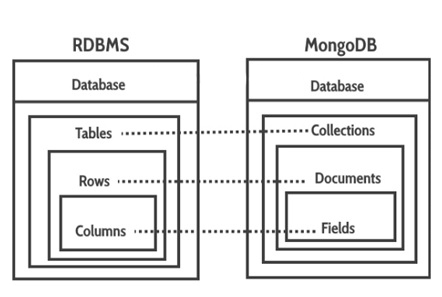
\includegraphics[scale=1.2]{mongodb-structure.jpg}
                \caption{Comparación de estructura de datos entre MongoDB y los RDBMS (sistema de gestión de bases de datos relacionales)}
            \end{figure}
        \fi

    \subsection{Fastify}

        Fastify es un framework web para Node.js de código abierto concentrado en proporcionar el mejor rendimiento, y una arquitectura flexible.

        Si comparamos la velocidad de fastify con otros frameworks web como express, tal como podemos ver en la figura \autoref{fig:fastify_vs_express}, notamos que fastify es aproximadamente un 20\% más rápido que express.

        \begin{figure}
            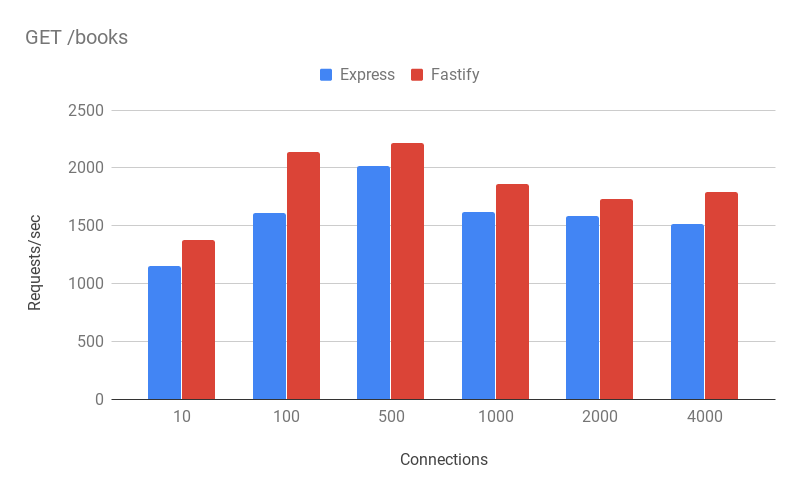
\includegraphics[scale=0.5]{fastify_vs_express.png}
            \caption{ Número de peticiones por segundo para distinta cantidad de conexiones}
            \label{fig:fastify_vs_express}
        \end{figure}
    


\section{Metodología de desarrollo}

    \subsection{Desarrollo Rápido de Aplicaciones (RAD)}

    El desarrollo rápido de aplicaciones es una metodología de desarrollo que prioriza la creación rápida y prototipos y la retroalimentación rápida sobre ciclos prolongados de desarrollo y prueba. Con el uso de RAD, los desarrolladores pueden realizar multiples iteraciones y actualizaciones al software rápidamente sin la necesidad de iniciar un cronograma de desarrollo desde cero cada vez.

    Esta metodología de desarrollo fue creada por James Martin en el año 1980 en IBM y fue formalizada con la publicación del libro \emph{Rapid Application Development} en 1991.

    \begin{figure}
        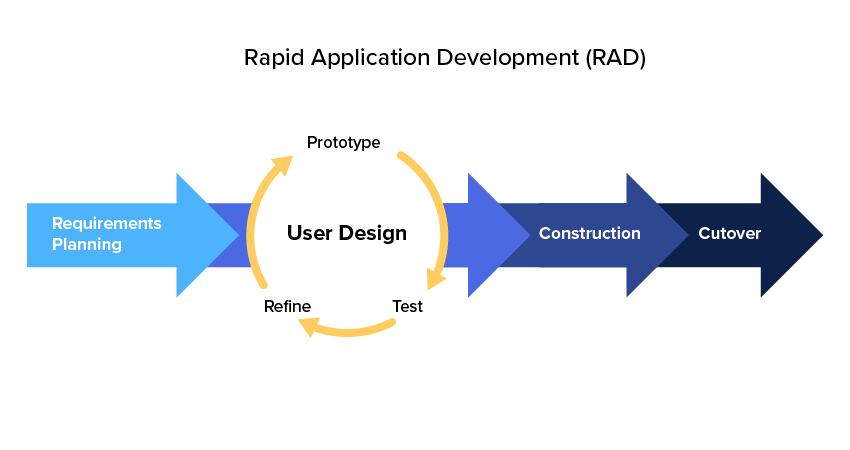
\includegraphics[scale=0.45]{Rapid-application-development.png}
        \caption{Fases del Desarrollo Rápido de Aplicaciones (enfoque de James Martin)}
        \label{fig:Rapid-application-development}
    \end{figure}

    \subsubsection{Fases del Desarrolo Rápido de Aplicaciones}

    Según el enfoque de James Martin el Desarrollo Rápido de Aplicaciones se divide en las siguientes fases \cite{RADJamesMartin}:

    \begin{itemize}
        \item \textbf{Fase de planificación:} Esta fase es equivalente a una reunión de alcance del proyecto. Aunque la fase de planificación se condensa en comparación con otras metodologías de gestión de proyectos.

        Durante esta etapa, los desarrolladores, los clientes (usuarios de software) y los miembros del equipo se comunican para determinar los objetivos y las expectativas del proyecto, así como los problemas actuales y potenciales que deben abordarse durante la construcción.

        \item \textbf{Fase de diseño:} Durante esta fase, los usuarios interactúan con analistas de sistemas y desarrollan modelos y prototipos que representan todos los procesos, entradas y salidas del sistema.
        
        Todos los errores y problemas se resuelven en un proceso iterativo. El desarrollador diseña un prototipo, el cliente (usuario) lo prueba y luego se reúnen para comunicar qué funcionó y qué no.
        
        \item \textbf{Fase de construcción:} Esta etapa toma los prototipos y el sistema en su fase beta resultado de la etapa de diseño y lo convierte en un modelo funcional.
        
        Debido a que la mayoría de los problemas y cambios se abordaron durante la minuciosa fase de diseño iterativo, los desarrolladores pueden construir el modelo de trabajo final más rápidamente que siguiendo un enfoque tradicional de gestión de proyectos.
        
        \item \textbf{Fase de transición:} Esta es la fase de implementación donde el producto terminado va al lanzamiento. Incluye conversión de datos, pruebas y cambio al nuevo sistema, así como capacitación de usuarios.

        Todos los cambios finales se realizan mientras los programadores y los clientes continúan buscando errores en el sistema.

    \end{itemize}





